\section{Vergleichbare Arbeiten und Produkte}
\label{sec:related-work}

Andere Entwicklungsumgebungen für Datenbanken, Konzepte zur Einführung in die Programmierung und auch Generatoren für Abfragemasken gibt es in schier unüberblickbarer Zahl. Dieses Kapitel stellt einige der vefügbaren Programme oder Bücher und hebt dabei insbesondere den Einfluss hervor, den sie auf \idename{} direkt oder indirekt genommen haben. Sinn dieses Kapitels ist damit der "`Blick über den Tellerrand"' um aus der Vielzahl an verfügbaren Ideen jene herauszustellen die für diese Arbeit von Bedeutung sind. Es handelt sich nicht um eine strukturierte Bewertung oder Einordnung dieser Inspirationsquellen.

\newpage

\subsection{Software: Scratch}

\begin{figure}[p]
  \centering 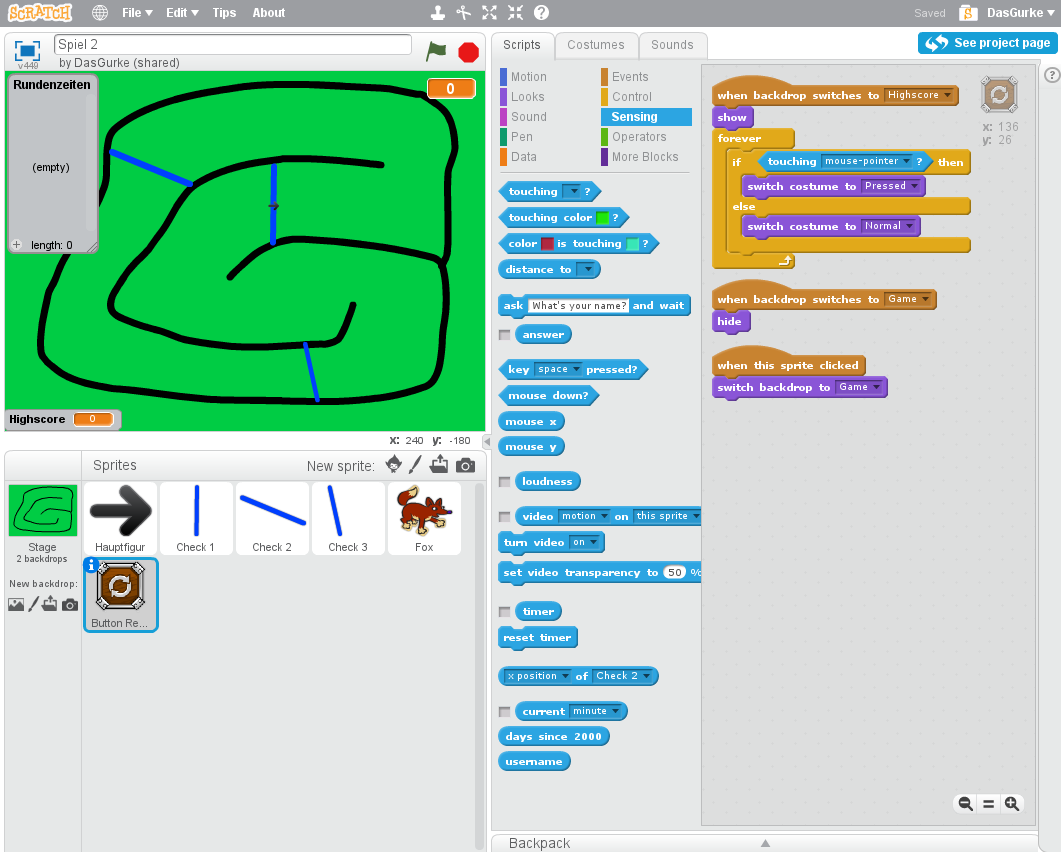
\includegraphics[width=\textwidth]{images/related-work-scratch-editor-full.png}
  \caption{Der Scratch-Editor mit einem Beispielprojekt aus Sicht eines Entwicklers}
  \label{fig:scratch-editor-full}
\end{figure}

\begin{figure}[p]
  \centering 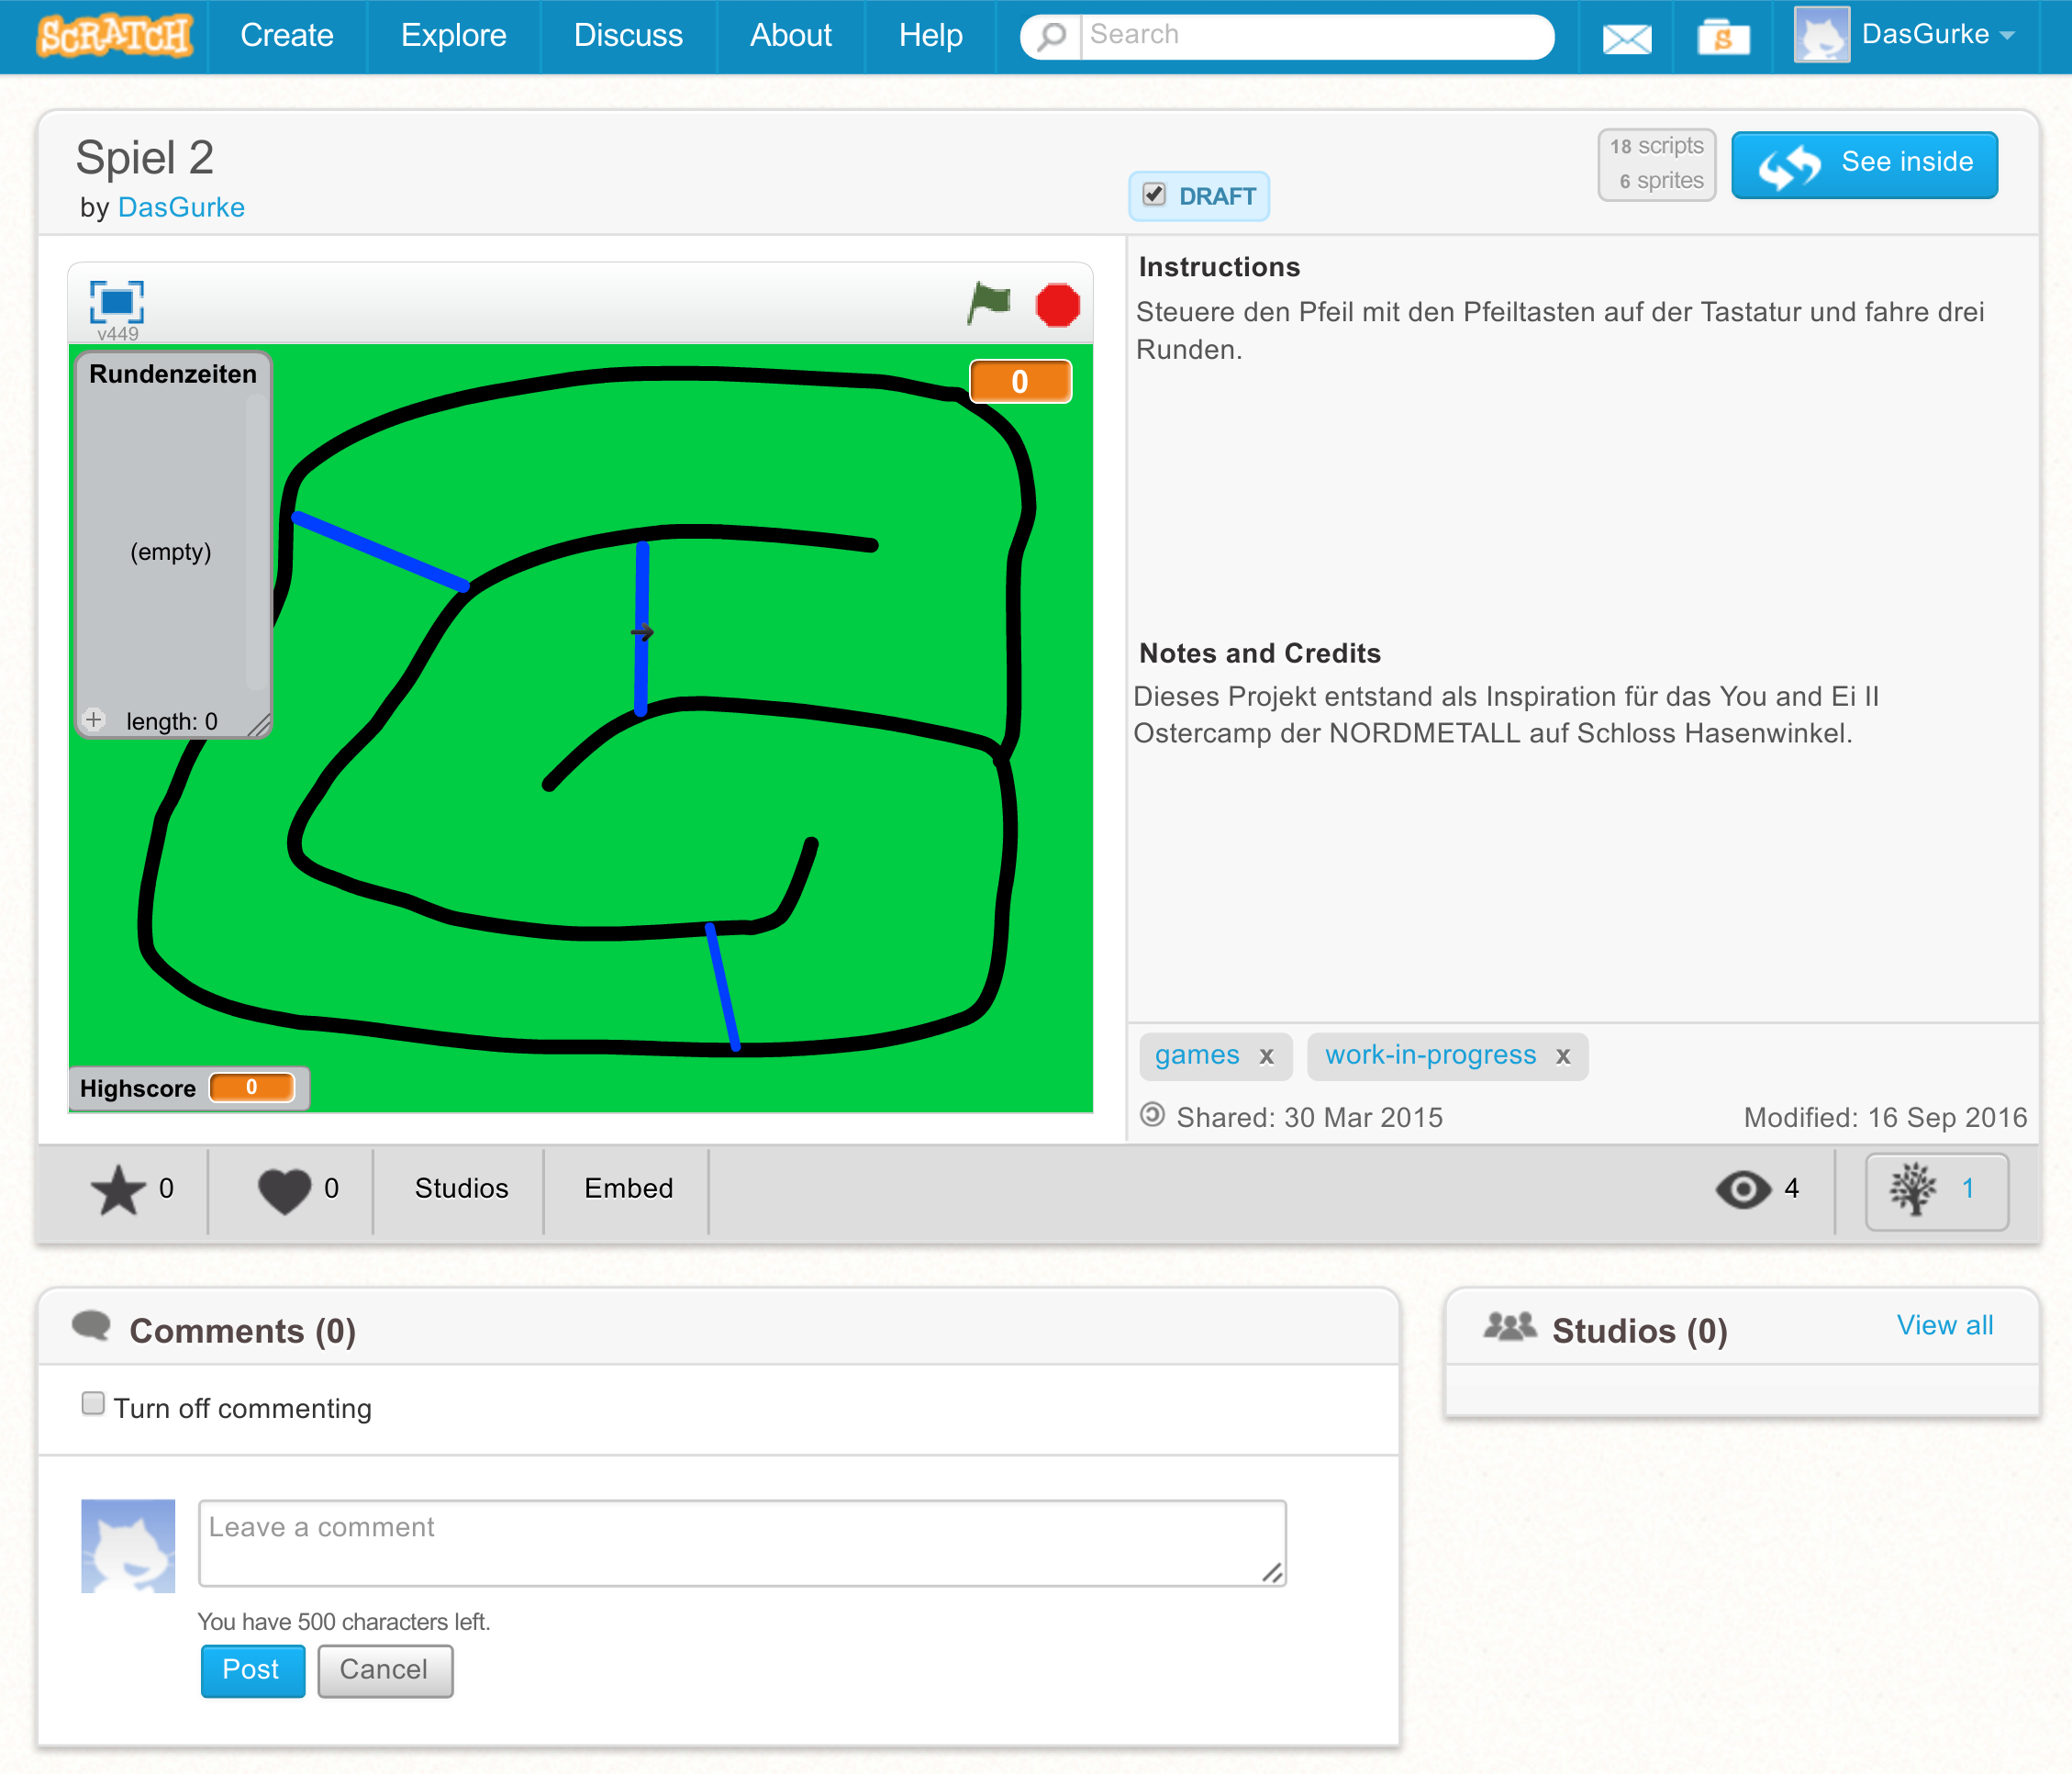
\includegraphics[width=0.8\textwidth]{images/related-work-scratch-project-full.png}
  \caption{Ein Scratch Projekt mit kurzen Handlungsanweisungen und einem Kommentarbereich in der Sicht für Endanwender.}
  \label{fig:scratch-enduser-full}
\end{figure}

Diese Masterarbeit zieht eine Menge Inspiration aus dem Scratch-Project des Massachusetts Institute of Technology (MIT)\footnote{Verfügbar als Download- und Webversion unter \url{https://scratch.mit.edu/}}. Bei Scratch handelt es sich um eine Entwicklungsumgebung speziell für Kinder und Jugendliche deren bestimmendes Bedienkonzept eine visuelle Programmiersprache ist. Scratch lehrt den Umgang mit imperativen und ereignisorientierten Programmierkonzepten und ist damit in Bezug auf die zu vermittelnden Inhalte recht weit dieser Thesis entfernt.

Im weiteren Verlauf der Arbeit wird dennoch deutlich werden, dass sich \idename{} an vielen Stellen sehr stark an Scratch orientiert. So nutzt auch \idename{} einen Drag \& Drop Editor um Syntaxfehler von vornerein auszuschließen und kontextsensitiv mögliche Operationen hervorzuheben. Die Verwendung eines, zu diesem Zeitpunkt allerdings nicht vollständig ausgearbeiteten, Farbkonzeptes nimmt sich ebenfalls Scratch zum Vorbild. Und schließlich ist auch die Zweiteilung eines Projekts in eine Besucheransicht sowie eine Entwickleransicht und der Wechsel zwischen diesen Modi eine direkte Inspiration.

Scratch baut dabei nicht auf einer bestehenden Programmiersprache auf, sondern nutzt eine Eigenentwicklung. Die Schlüsselwörter dieser Sprache, wie auch die Oberfläche des Editors, sind dabei in viele verschiedene natürliche Sprachen (Englisch, Deutsch, Spanisch, ...) übersetzt worden. Abbildung \ref{fig:scratch-editor-full} zeigt wie diese Sprache innerhalb des Scratch-Editors für einen Entwickler aussieht. Mit Scratch entwickelte Programme basieren in der Regel darauf, Figuren über eine Zeichenfläche zu verschieben. Dementsprechend gut eignet sich Scratch zur Entwicklung kleinerer Spiele, die Werte von Variablen (Position, Orientierung, Größe, ... von Objekten) können sehr gut veranschaulicht und damit vergleichsweise intuitiv erfasst werden.

Abbildung \ref{fig:scratch-enduser-full} demonstriert wie sich ein Projekt initial einem Endanwender präsentiert. Als Entwickler gibt man einem Projekt einen Namen, eine kurze Beschreibung und erwähnt möglicherweise Helfer und Inspirationsquellen. Besucher können über eine Kommentarfunktion Rückmeldung geben.

\newpage

\subsection{Software: App Inventor}

Bei dem AppInventor\footnote{Verfügbar unter \url{http://appinventor.mit.edu/}} handelt es sich um eine Kollaboration des MIT mit Google und gewissermaßen um eine logische Fortführung von Scratch. Erstellt werden mit dem AppInventor nicht mehr in Webseiten einbettbare Flash-Anwendungen, sondern Apps für das Android Betriebssystem. Wie schon Scratch läuft auch diese Anwendung in einem Webbrowser. Grundsätzlich ist auch diese Webseite in verschiedenen Sprachen verfügbar, Deutsch zählt zum gegenwärtigen Zeitpunkt allerdings nicht dazu.

Im Vergleich zu Scratch ist der AppInventor wesentlich anspruchsvoller, die Struktur der relativ komplizierten Android-Oberflächen wird vor dem Benutzer nicht versteckt, dafür aber in einen WYSIWYG-Editor verpackt\footnote{"`What You See Is What You Get"' bezeichnet die visuelle Vorschau in einem Editor ohne den Umweg über einen Kompilierungsschritt.}. Der zu schreibende Programmcode wird, wie schon bei Scratch, in einer abstrakten Sprache mit Drag \& Drop Elementen formuliert. Daraus wird dann Java-Code erzeugt, diesen bekommt der Entwickler im Normalfall aber nicht zu Gesicht.

\begin{figure}[h]
  \centering 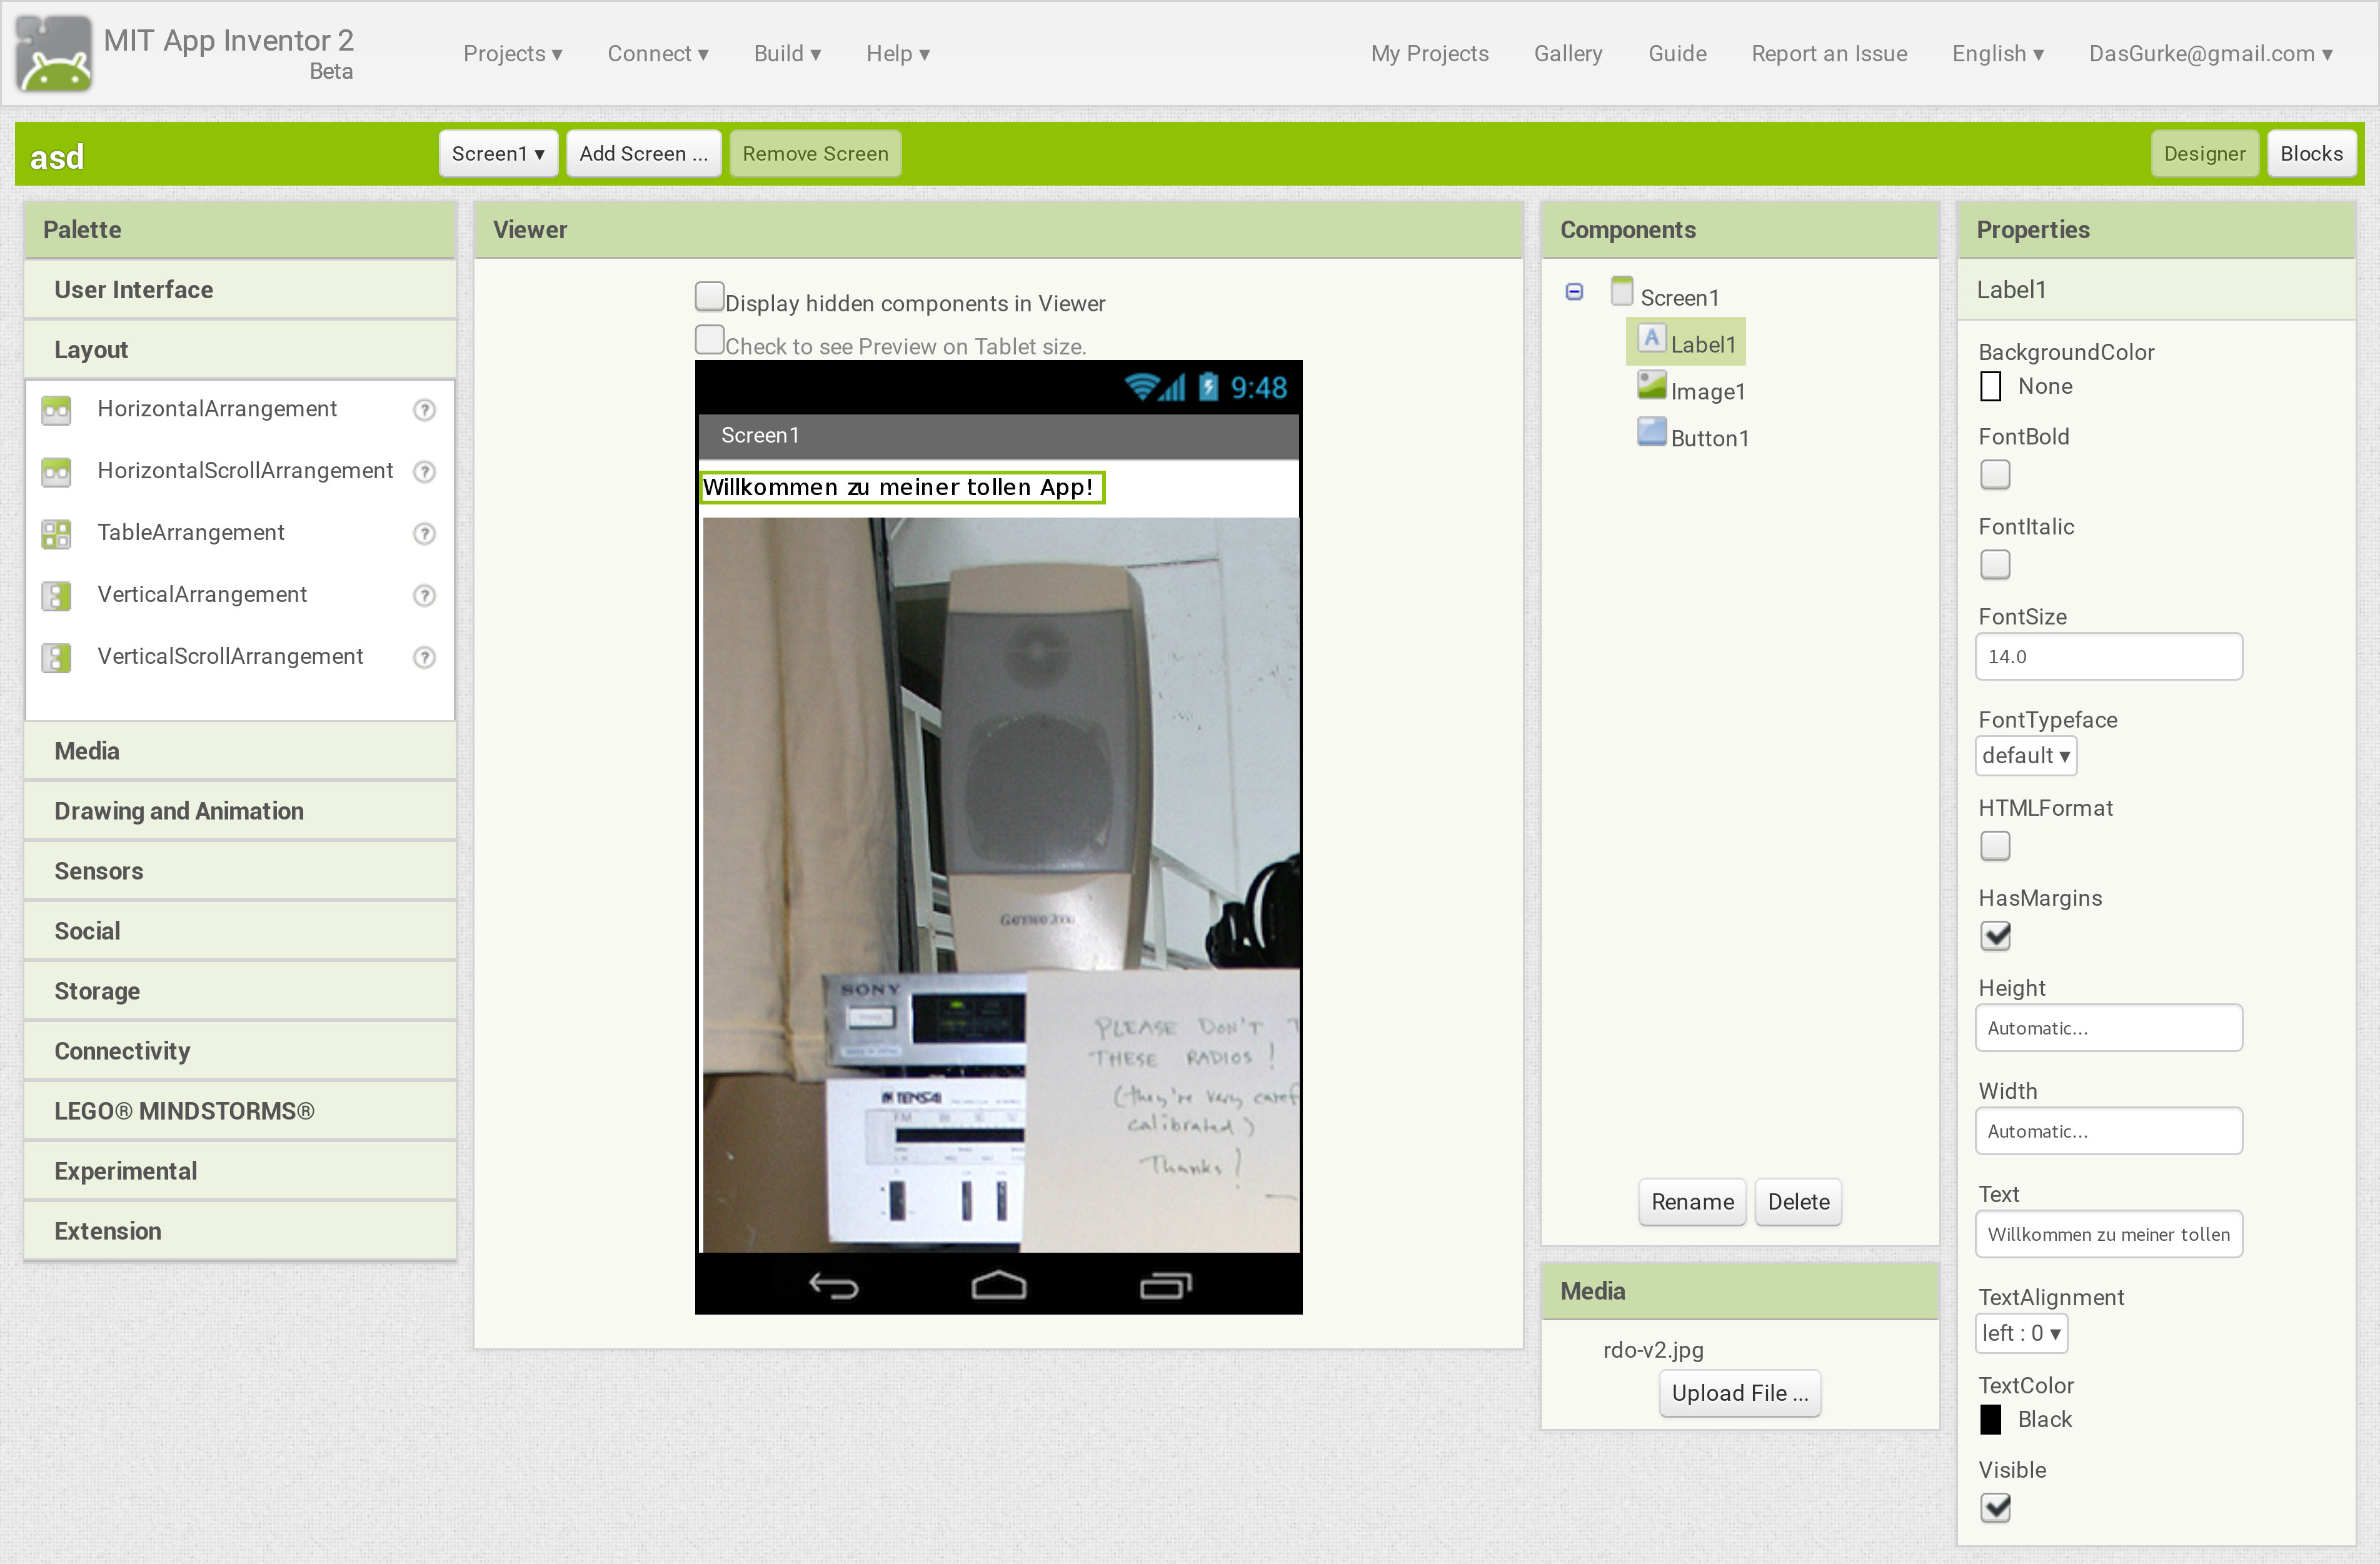
\includegraphics[width=\textwidth]{images/related-work-app-inventor-designer.png}
  \caption{Oberflächeneditor des App Inventor}
  \label{fig:app-inventor-ui-designer}
\end{figure}

\begin{figure}[h]
  \centering \includegraphics[width=\textwidth]{images/related-work-app-inventor-blocks.png}
  \caption{Codeeditor des App Inventor.}
  \label{fig:app-inventor-block-designer}
\end{figure}

Um die Anwendungen zu testen müssen diese auf das Handy der Entwickler geladen oder in einem Emulator ausgeführt werden. Es ist dafür nötig, ein (reales oder emuliertes) Gerät über die "`App Inventor Companion App"' direkt mit der Webseite zu verbinden. Sobald diese Verbindung steht werden die im Browser vorgenommenen Änderungen mit einer kurzen Verzögerung auf dem Smartphone widergespiegelt.

Wie Scratch befördert auch der App Inventor den Austausch von Entwicklern untereinander. Es ist möglich die eigenen Apps in einer Gallerie auszustellen und dort zu den Entwicklungen von anderen Menschen Rückmeldung zu geben. Die Arbeitsergebnisse sind dabei häufig sehr datenorientiert: Die Vorauswahl an verfügbaren Bedienelementen umfasst zwar neben typischen Bedienelementen wie Textfeldern oder Auswahllisten auch grafische Komponenten wie Bälle oder Zeichenflächen. Der Umgang mit diesen Elementen ist im Vergleich zu Scratch alleine durch den im direkten Vergleich wesentlich langsameren Rückmeldezyklus wesentlich anspruchsvoller. Um korrekte Ergebnisse zu erhalten ist es notwendig sich schon im Voraus recht viele Gedanken zu machen.

Auch aufgrund der schieren Masse an möglichen Bedienelementen und den teilweise sehr unterschiedlichen darauf definierten Operationen wird der Komplexitätsgrad merklich gesteigert. Anders als bei Scratch kann man sich nicht mehr ohne weiteres durch eine sehr begrenzte Anzahl von Möglichkeiten durchklicken und sich am Ende halbwegs sicher sein nun auch alles gesehen zu haben. Dieser erhöhte Komplexitätsgrad ist dabei selbstverständlich nicht nur als Nachteil zu verstehen: Man richtet sich mit dem App Inventor an eine fortgeschrittenere Zielgruppe als jene von Scratch.

\subsection{Kurs: SqlZoo}

Bei der Webseite "`SqlZoo"'\footnote{Verfügbar unter \url{http://sqlzoo.net/}} handelt es sich sowohl um einen Kurs in Form einer Sammlung von aufeinander aufbauenden Aufgaben inklusive begleitendem Lehrmaterial, als auch eine webbasierte Software in welcher die Lernenden ihre ersten Schritte mit SQL machen. Anders als in Scratch erfolgt die Programmierung der nötigen Abfragen in einem normalen Textfeld und "`echtem"' SQL. Syntax-Hervorhebung oder andere unterstützende Hilfsmittel wie automatische Code-Formatierung sind nicht vorhanden.

Dem Lernenden präsentiert sich das Projekt ähnlich wie ein Lehrbuch mit Übungsaufgaben. Diese sind thematisch in Kapitel untergliedert und nutzen in der Regel einen sehr überschaubaren Datenbestand. Die Ergebnisse werden neben dem Textfeld angezeigt und können mit dem korrekten Ergebnis verglichen werden (Abbildung \ref{fig:sqlzoo-check-result}). So können Lernende ihre Ergebnisse selbständig kontrollieren.

\begin{figure}[h]
  \centering \includegraphics[width=\textwidth]{images/related-work-sql-zoo-error.png}
  \caption{Technische Fehlermeldung einer Datenbank aufgrund eines Syntaxfehlers in der Eingabemaske von SqlZoo.}
  \label{fig:sqlzoo-check-result}
\end{figure}

Nach den Lerneinheiten folgt dann eine Serie von Quizfragen (Abbildung \ref{fig:sqlzoo-quiz-sql-formalization}). Dabei handelt es sich um multiple choice Aufgaben, es müssen keine SQL-Abfragen geschrieben werden. Primär wird bei diesen Fragen eine Zuordnung verlangt: Dem Lernenden wird wahlweise eine Ergebnismenge oder eine Abfrage gezeigt und es muss die jeweils passende Abfrage oder Ergebnismenge dazu identifiziert werden. Weitere Aufgabentypen beschäftigen sich zum Beispiel mit der Wahl der korrekten SQL-Formalisierung zu einer natürlichsprachlich formulierten Anfrage.

\begin{figure}[h]
  \centering 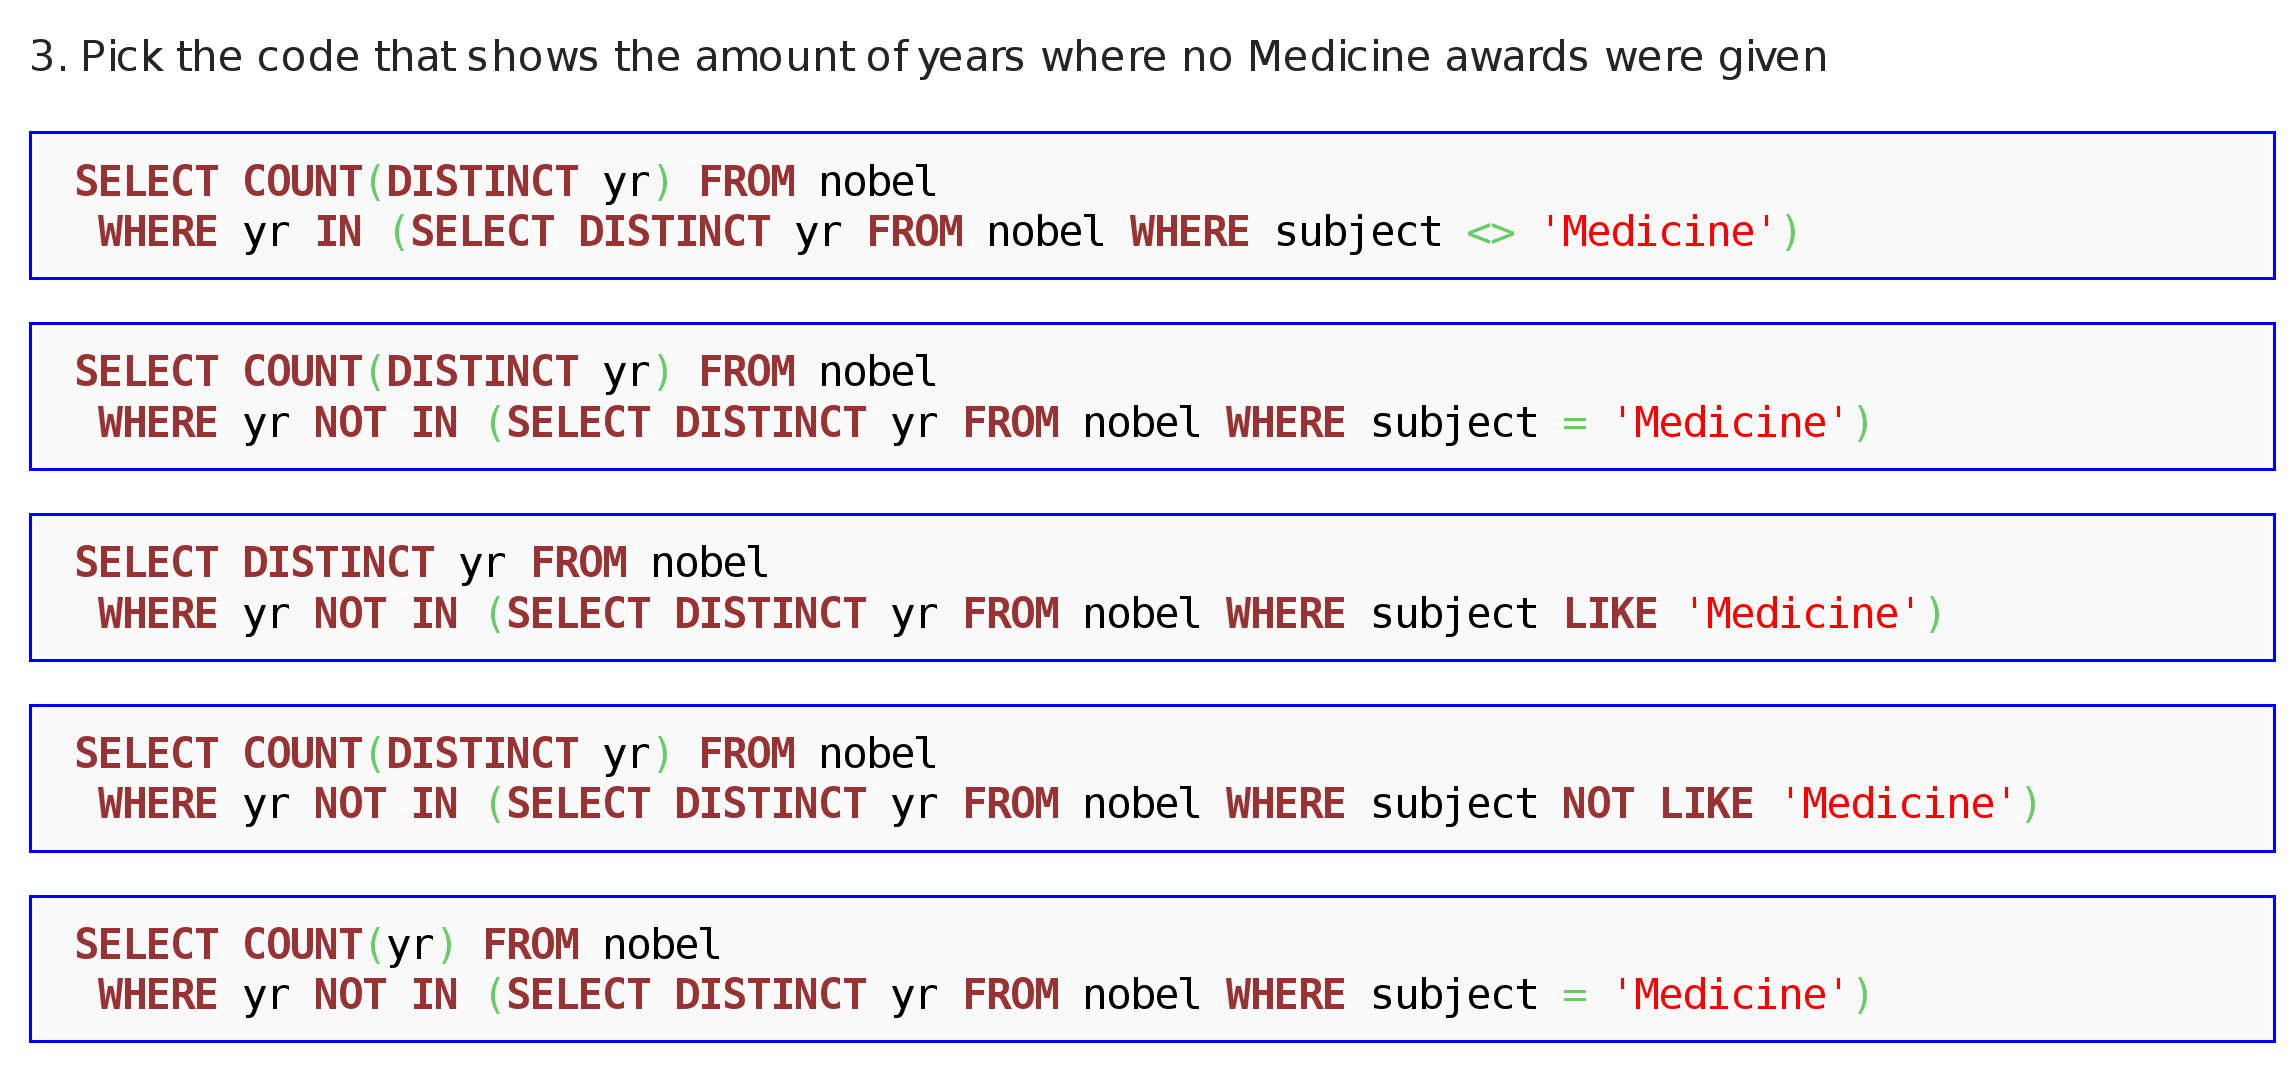
\includegraphics[width=\textwidth]{images/related-work-sql-zoo-quiz-select-sql.png}
  \caption{Quizfrage: Zu einer natürlichsprachigen Aussage muss die korrekte SQL-Formalisierung gewählt werden.}
  \label{fig:sqlzoo-quiz-sql-formalization}
\end{figure}

Ein Alleinstellungsmerkmal dieses Angebots ist die sehr breite Unterstützung verschiedener Datenbanksysteme. Als Lernender kann man die Aufgaben wahlweise mit dem Microsoft SQL Server, Oracle, MySQL, DB2, Ingres oder PostgreSQL lösen. SqlZoo wir ebenfalls in mehreren Sprachen angeboten, die deutsche Übersetzung ist allerdings nicht durchgehend verfügbar.

Es ist mit dem SqlZoo prinzipiell auch möglich mutierende Abfragen auszuführen. Diese werden im Normalfall allerdings nicht über eine einmalige Anzeige hinaus persistiert. Angemeldete Benutzer können zwar auch eigene Tabellen anlegen, agieren damit aber immer in einem globalen Namensraum ohne differenzierte Zugriffskontrollen: Es ist jedem bearbeitenden Nutzer möglich beliebige Datenbestände zu verändern. Alle mutierenden Operationen, es wird zum Beispiel auch \lstinline{CREATE TABLE} behandelt, sind dabei aktuell lediglich als Referenz verfügbar und nicht Teil des Kursangebotes mit dezidierten Quizaufgaben.

Auch wenn es durch den Wiki-Unterbau von SqlZoo den Lernenden theoretisch möglich wäre eigene Projektideen innerhalb der Webseite umzusetzen, ist das eindeutig nicht das Ziel des Angebotes. Anders als bei Scratch oder dem App Inventor steht am Ende dieses Angebotes also keine eigene Software, sondern Erkenntnisgewinn.

\subsection{Software: Jekyll}
\label{sec:software-jekyll}
Bei Jekyll\footnote{Dokumentation verfügbar unter \url{http://jekyllrb.com/}} handelt es sich um ein quelloffenes Framework zur Erstellung statischer Webseiten. Der Begriff "`statisch"' bezeichnet in diesem Kontext das Ergebnis der Kompilierung: HTML Seiten, die von jedem Webserver unverändert ausgegeben werden können. Technisch gesehen setzt Jekyll auf die HTML-Templatingsprache Liquid auf und stellt während der Generierung einer Seite eine Vielzahl von hilfreichen Metadaten bereit. Diese Metadaten werden entweder implizit aus Dateinamen gewonnen oder in YAML-Notation im Kopf einer Datei definiert.

In der Standardkonfiguration eignet sich Jekyll vor allem um ohne großen Aufwand eine Blog-artige Seite zu betreiben. Alle Dateien die sich in einem speziellen Ordner \lstinline{_posts} befinden werden als Datenquelle für Blogeinträge behandelt. Ein solcher Eintrag könnte dabei aussehen wie in Listing~\ref{lst:jekyll-post}, typischerweise würden natürlich mehrere solcher Dateien für Beiträge existieren. Bei dem Bereich zwischen den \lstinline{---} handelt es sich um das so genannte "`YAML-Frontmatter"'. Diese Metadaten stehen dem Entwickler im Kontext dieser Seite zur Verfügung. Um diese in die Seite einzubetten werden sie als Liquid-Ausdruck in geschweifte Klammer
n geschrieben.

Einige der Metadaten werden von Jekyll ausgewertet, zum Beispiel \lstinline{layout}. Dabei handelt es sich um das Liquid-Template, welches einen solchen Beitrag darstellen soll. Wie ein solches Template aussieht zeigt Listing~\ref{lst:jekyll-post-template}. Auch dieses Layout wird seinerseits wieder in ein anderes Layout eingebettet, der Ausdruck \lstinline|{{ content }}| bezeichnet dabei den Ort an dem diese Einbettung stattfindet. Listing~\ref{lst:jekyll-master-template} zeigt wie Kette von Einbettungen in einer letzten Vorlage endet. Ziel dieser Einbettung ist die Vermeidung von Redundanzen: Um zum Beispiel auf allen Seiten eine neue CSS-Datei zu referenzieren muss in diesem Beispiel nur Listing~\ref{lst:jekyll-master-template} angepasst werden.

\begin{lstlisting}[float=p,caption={Ein Blogbeitrag mit Metadaten für Jekyll} ,label={lst:jekyll-post}]
---
layout: post
title: So funktioniert Jekyll
categories: [simple,beginner]
author: Marcus
test: 3.141
---
Dies ist ein einfacher Blogeintrag mit wenigen Metadaten. Das Datum des
Beitrages wird aus dem Dateinamen generiert. {{ page.test }} ist ein
Wert der testweise ausgegeben wird.
\end{lstlisting}

\begin{lstlisting}[float=p,caption={Beispieltemplate für Blogbeiträge für Jekyll}, label={lst:jekyll-post-template}]
---
layout: default
---
<h2>{{ page.title}} <small>von {{ page.author}}</small></h2>
<ul>
  
    <li>{{ category }}</li>
  
</ul>
<div class="content">
  {{ content }}
</div>
\end{lstlisting}

\begin{lstlisting}[float=p,caption={Template mit HTML-Rumpf für Jekyll}, label={lst:jekyll-master-template}]
<html>
  <head><title>{{ site.title }} - {{ page.title }}</title></head>
  <body>
    {{ content }}
  </body>
</html>
\end{lstlisting}

\begin{lstlisting}[float=p,caption={Hauptseite mit Auszügen aller Beiträge für Jekyll}, label={lst:jekyll-main-page}]
---
layout: default
---
<h1>{{ site.title }}</h1>

  <div>
    <a href="{{ post.url }}">{{ post.title }}</a>
    {{ post.excerpt }}
  </div>

\end{lstlisting}

Die Metadaten werden von Jekyll in unterschiedliche Namensräume gruppiert. Globale Daten werden in einer speziellen YAML-Datei hinterlegt und können über das Präfix \lstinline{site} addressiert werden. Daten zu spezifischen Seiten erhalten das Präfix \lstinline{page}.

Um nun auf einer Hauptseite alle Beiträge anzuzeigen stellt Jekyll im \lstinline{site} Namensraum eine spezielle Liste names \lstinline{posts} zur Verfügung. Diese können dazu genutzt werden alle Blogbeiträge auf einer Hauptseite anzuzeigen. Listing~\ref{lst:jekyll-main-page} zeigt wie der Code für eine solche Seite aussehen könnte. Die Eigenschaften \lstinline|page.url| und \lstinline|page.excerpt| werden dabei automatisch von Jekyll generiert.

Die Generierung von Webseiten in \idename{} ist stark von Jekyll inspiriert. Die offensichtlichste Gemeinsamkeit ist die Nutzung der gleichen Templating-Engine "`Liquid"', aber auch das Datenmodell und dessen Aufteilung in verschiedene Namensräume wurde von Jekyll inspiriert. In einer der ersten Prototypen handelte es sich bei \idename{} sogar um ein Plugin für Liquid, welches im Kopfbereich definierte SQL-Abfragen auswertete und im Kontext der Seiten zur Verfügung stellte. Die statische Natur der von Jekyll generierten Seiten disqualifiziert es allerdings als Kandidat für eine softwaretechnische Basis von \idename{}.

\subsection{Software: Visual Studio Lightswitch}

Diese Variante des Microsoft Visual Studio ist auf die Entwicklung von datenoriertieren Geschäftsanwendungen ausgelegt. Sie erlaubt eine schnelle Integration von heterogenen Datenquellen und erstellt Anwendungen, die entweder als Silverlight-Desktopanwendung oder im Browser laufen.

Visual Studio Lightswitch richtet sich vornehmlich an Informatik-affine Mitarbeiter, die jedoch im Regelfall jedoch nicht zwingend über eine formale Informatik-Ausbildung verfügen. Es kann gewissermaßen als der logische nächste Schritt nach dem Datenbanksystem Microsoft Access gesehen werden. Die Programmierung dieser Anwendungen erfolgt in den normalen Editoren für Javascript oder C\# des Visual Studio. Beide Sprachen sind prinzipiell im vollen Umfang verfügbar, es existiert keine gesonderte Unterstützung um Anfängern die ersten Schritte zu erleichtern oder typische Fehler zu lokalisieren. Eine Vereinfachung ergibt sich durch die spezialisierte Programmierschnittstelle, welche die Verknüpfung unterschiedlicher Datenquellen mit der Oberfläche erleichtern.

Es gibt unterschiedliche Arten und Weisen um innerhalb einer Lightswitch-Anwendung auf Daten zuzugreifen, im Rahmen dieser Arbeit ist aber lediglich der Umgang mit Datenbanken von Bedeutung. Für diese existiert ein eigener Editor (Abbildung \ref{fig:lightswitch-data-designer}), welcher es erlaut die Spalten einzelner Tabellen zu editieren und Beziehungen einzufügen. Die benötigten C\#-Klassen werden dann automatisch erzeugt und mittels eines Objekt-Relationalen-Mappers (ORM) auf die Struktur der Datenbank gemappt. Diese Vorgehensweise führt dabei zu einer Einschränkung, die im Lehrkontext zumindest ärgerlich ist: \lstinline{m:n}-Beziehungen zwischen Objekten können nicht erstellt werden, sondern müssen manuell durch zwei \lstinline{1:n}-Beziehungen mit einer "`künstlichen"' Entität in der Mitte abgebildet werden.

\begin{figure}[h]
  \centering \includegraphics[width=\textwidth]{images/related-work-lightswitch-data-editor.png}
  \caption{Schemaeditor von Visual Studio Lightswitch}
  \label{fig:lightswitch-data-designer}
\end{figure}

Die Oberflächen werden in einem Editor erstellt, welcher die Hierarchie der Bedienelemente in einem Baum visualisiert (Abbildung \ref{fig:lightswitch-ui-designer}). Es stehen abhängig von der Zielplattform (Browser oder Desktop) im Detail unterschiedliche, aber in der Programmierung sehr ähnliche Bedienelemente bereit. Wichtigstes Element ist dabei die sehr mächtige Visualisierung von tabellarischen Daten.

\begin{figure}[h]
  \centering 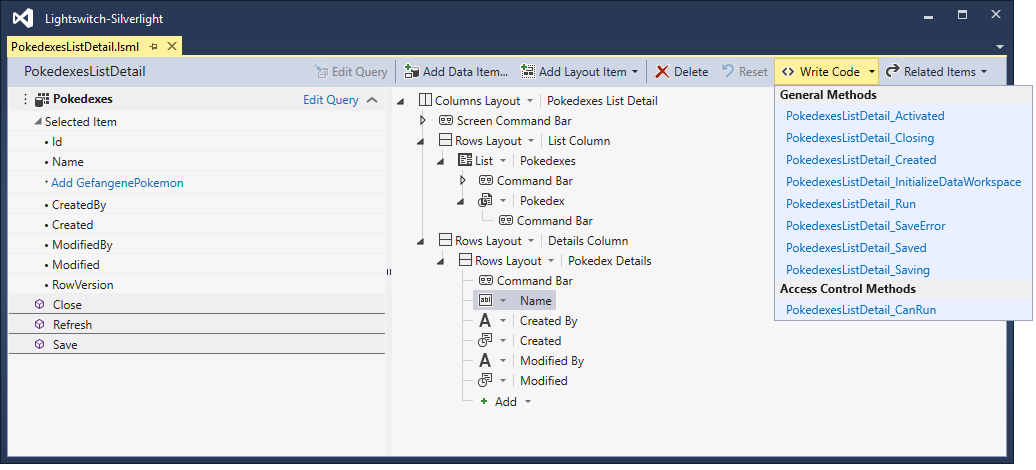
\includegraphics[width=\textwidth]{images/related-work-lightswitch-ui-editor.png}
  \caption{Oberflächeneditor von Visual Studio Lightswitch}
  \label{fig:lightswitch-ui-designer}
\end{figure}

Beide Editoren erlauben die Implementierung von speziellen Methoden, welche den CRUD-Zyklus oder spezielle Ereignisse innerhalb der Oberfläche abbilden. Es ist zwar auch möglich, Code außerhalb dieser vordefinierten Struktur zu schreiben, dieser kann dann aber nicht unmittelbar in den Editoren referenziert werden.

Ein Lightswitch-Projekt gliedert sich in zwei wesentliche Unterstrukturen: Datenquellen und Beschreibungen von Oberflächen. Diese werden auf zwei Projekte für Server und Client aufgeteilt, das Datenmodell ist jedoch transparent auf beiden Seiten verfügbar. Diese klare Trennung zwischen Datenmodell und Visualiserung findet sich auch bei \idename{} wieder.

\subsection{Buch: Die Macht der Abstraktion}

Bei diesem Buch von Herbert Klaeren und Michael Spaerber wird ein sehr von Datenstrukturen geprägter Ansatz zur Einführung in die Programmierung gewählt. Die Autoren beschreiben die gängigen Programmiersprachen aufgrund ihrer umfangreichen Syntax als ungeeignet für die Einführung in die Programmierung \cite[2]{macht-der-abstraktion}. 

Folglich unterrichtet das Buch auch nicht Java, C\#, Python, Ruby oder Pascal. Stattdessen kommt der Scheme-Dialekt ``Racket'' zum Einsatz. Bei Scheme handelt es sich wiederrum um einen der wesentlichen Varianten von Lisp, einer Programmiersprache deren Syntax fast exklusiv auf der Verwendung von runden Klammern zur Beschreibung von Tupeln aufbaut. Durch diese sehr reduzierte Syntax versprechen sich die Autoren die Vermeidung von typischen syntaktischen Stolperfallen, mit denen Lernende zu Beginn oft Schwierigkeiten haben.

Die Anpassung an eine für Lernende gut geeignete Umgebung geht allerdings über diese vergleichsweise simple Syntax hinaus: Der Sprachumfang von Racket selbst wird im Laufe des Buches mehrfach erweitert. Abbildung~\ref{fig:drracket-language-levels} zeigt den Auswahldialog der ``Dr Racket''-Umgebung, in welchem auch die zum Buch passenden Sprachumfänge verfügbar sind.

\begin{figure}[h]
  \centering \includegraphics[width=\textwidth]{images/related-work-drracket-language-levels.pdf}
  \caption{Verfügbare Sprachniveaus in ``Dr Racket''}
  \label{fig:drracket-language-levels}
\end{figure}

\subsection{Software: MySQL Workbench}

Die MySQL Workbench ist das hauseigene Management- und Verwaltungsprogramm des gleichnamigen Datenbanksystems. Es unterstützt Programmierer mit speziellen Funktionen zur Modellierung von Datenbanken oder beim Entwickeln von Abfragen zu existierenden Datenbeständen. Systemadministratoren haben mit der Workbench Zugriff auf Performance-Indikatoren wie Caching-Fehlerraten, Datendurchsatz oder sonstige Auslastungsmerkmale.

Anders als das Visual Studio Lightswitch unternimmt die MySQL Workbench keinerlei Versuche technische Details vor dem Anwender zu verstecken. Es handelt sich im wesentlichen um eine grafische Benutzerschnittstelle für jene Daten, die ebenso von der Programmierschnittstelle bereitgestellt werden.

Da es sich um ein spezialisiertes Programmes eines Datenbanksystems handelt, bietet der Schema-Designer (Abbildung~\ref{fig:mysql-workbench-schema-diagram}) keinerlei Unterstützung für konzeptuelle (z.B. mit Entity-Relationship-Modellen) Modellierung. Er beschäftigt sich ausschließlich mit der Darstellung oder Modifikation von physikalischen Modellen. Im Editor stehen zwar Komfortfunktionen für die Modellierung von Beziehungen aller typischen Kardinalitäten zur Verfügung, diese werden aber unmittelbar auf Fremdschlüssel und gegebenenfalls Kreuztabellen abgebildet. Von $m:n$-Beziehungen wird folglich nicht abstrahiert, sondern stattdessen die gängige Abbildung in Form einer Kreuztabelle automatisch vorgenommen.

Der Editor für Abfragen bietet alle typischen Funktionen einer Entwicklungsumgebung (Abbildung~\ref{fig:mysql-workbench-query}): Dem Entwickler werden kontextsensitiv Vervollständigungsvorschläge angeboten, die Struktur der involvierten Tabellen ist in einer Seitenleiste sichtbar. Das Ergebnis der Abfrage wird in einem variabel großen Bereich unter dem Texteditor angezeigt. Und unter diesem Bereich wiederrum ist eine Historie der zuletzt ausgeführten Abfragen verfügbar.

Die Workbench versucht sowohl syntaktische (zum Beispiel fehlende Klammern) als auch logische (zum Beispiel nicht vorhandene Spalten) Fehler optisch hervorzuheben. Dafür werden die Abfragen anscheinend aber nicht gegen den Server validiert. Dadurch entstehen gelegentlich Inkonsistenzen in beide Richtungen: Es werden möglicherwereise Fehler im Editor angezeigt, welche auf dem Server nicht auftreten. Auch der umgekehrte Fall kann aber eintreten: Tatsächlich aufgetrene Fehler auf dem Server werden nicht mit einer entsprechenden Markierung im Editor versehen.

\begin{figure}[p]
  \centering \includegraphics[width=\textwidth]{images/related-work-mysql-workbench-db-diagram.png}
  \caption{Visueller Schema-Editor der MySQL Workbench}
  \label{fig:mysql-workbench-schema-diagram}
\end{figure}

\begin{figure}[p]
  \centering \includegraphics[width=\textwidth]{images/related-work-mysql-workbench-query.png}
  \caption{Abfrageeditor der MySQL Workbench}
  \label{fig:mysql-workbench-query}
\end{figure}

%%% Local Variables:
%%% mode: latex
%%% TeX-master: "thesis"
%%% End:
